\documentclass{standalone}
\usepackage{graphicx}	
\usepackage{amssymb, amsmath}
\usepackage{color}

\usepackage{tikz}
\usetikzlibrary{intersections, backgrounds, math, arrows.meta}
\usepackage{pgfmath}

\definecolor{light}{RGB}{220, 188, 188}
\definecolor{mid}{RGB}{185, 124, 124}
\definecolor{dark}{RGB}{143, 39, 39}
\definecolor{highlight}{RGB}{180, 31, 180}
\definecolor{light_teal}{RGB}{107, 142, 142}
\definecolor{mid_teal}{RGB}{72, 117, 117}
\definecolor{dark_teal}{RGB}{29, 79, 79}
\definecolor{gray10}{gray}{0.1}
\definecolor{gray20}{gray}{0.2}
\definecolor{gray30}{gray}{0.3}
\definecolor{gray40}{gray}{0.4}
\definecolor{gray60}{gray}{0.6}
\definecolor{gray70}{gray}{0.7}
\definecolor{gray80}{gray}{0.8}
\definecolor{gray90}{gray}{0.9}
\definecolor{gray95}{gray}{0.95}

\tikzmath{
}

\begin{document}

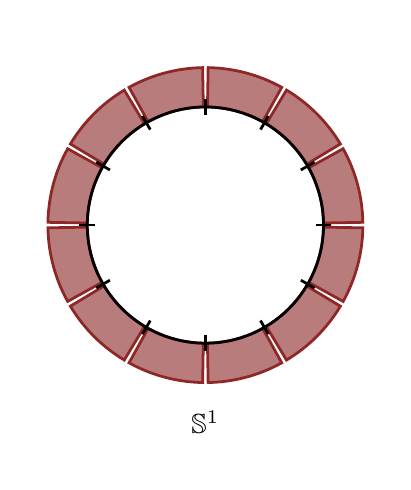
\begin{tikzpicture}[scale=1.0]

  \begin{scope}[shift={(0, 0)}]
    \draw[white] (-2.25, -3) rectangle (2.25, 2.5);
    
    \pgfmathsetmacro{\r}{1.5}
    \pgfmathsetmacro{\delta}{0.1}
    \pgfmathsetmacro{\dt}{1}
    \pgfmathsetmacro{\h}{0.5}
    
    \foreach \t in {0, 30, 60, ..., 330} {
      \filldraw[fill=mid, draw=dark, line width=1]    
          ( { \r * cos(\t + \dt) }, { \r * sin(\t + \dt) } )
       -- ( { (\r + \h) * cos(\t + \dt) }, { (\r + \h) * sin(\t + \dt) } ) arc ({\t + \dt}:{\t + 30 - \dt}:{\r + \h} )
       -- ( { \r * cos(\t + 30 - \dt) }, { \r * sin(\t + 30 - \dt) } )
       -- ( { \r * cos(\t + 30 - \dt) }, { \r * sin(\t + 30 - \dt) } ) arc ({\t + 30 - \dt}:{\t + \dt}:{\r} );
    }

    \draw[line width=1] (0, 0) circle (\r);
    
    \pgfmathsetmacro{\delta}{0.1}
    \foreach \t in {0, 30, 60, ..., 330} {
      \draw[line width=1]    ( { (\r - \delta) * cos(\t) }, { (\r - \delta) * sin(\t) } )
                          -- ( { (\r + \delta) * cos(\t) }, { (\r + \delta) * sin(\t) } );
    }
    
    \node at (0, -2.5) { $\mathbb{S}^{1}$ };
  \end{scope}
  
\end{tikzpicture}

\end{document}  